%!TEX root = ../BoYu-Dissertation.tex
\graphicspath{{Figures/}}

\chapter{Awareness Promotion} % (fold)
\label{cha:awareness_promotion}
This chapter provides the overview of our computational approach to supporting awareness in complex, distributed collaborative activities. Our approach aims to address the limitations in existing awareness support systems as we identified in last chapter. The general design principle of our approach is to emphasize the active role of computer system to not merely support, but rather promote awareness among collaborators.

In the following, we first present the design philosophies behind our awareness promotion approach, and then overview the awareness promotion approach and the corresponding computational framework. More details about our approach will be given in the following two chapters (Chapter \ref{cha:knowledge_reprsentation_and_updating} and \ref{cha:promoting_event_driven_awareness}).

\section{From awareness support to awareness promotion} % (fold)
\label{sec:from_awareness_support_to_awareness_promotion}
In order to address the unique challenges for supporting awareness in complex, distributed collaborative activities, we propose the awareness promotion approach to emphasize the active role of computer systems to mediate awareness among collaborators. Our awareness promotion approach has its basis in two basic parent disciplines:  artificial intelligence (AI) and human-computer interaction (HCI). 
\begin{enumerate}
   \item From AI, we consider the computer as \emph{an active agent} \cite{Brown99activeuser}, situated within the collaborative environment that adaptively sense, acts, and reacts within this environment over time, to pursue its goal of promoting awareness.
   \item From HCI, we act on the premise that computers and humans have fundamentally asymmetric abilities \cite{Dalal1994}; therefore, we focus on developing divisions of responsibility that exploit the strengths and overcome the weaknesses of both, and utilizing interaction techniques to facilitate effective \emph{human-computer collaboration} \cite{Terveen1995}.
\end{enumerate}

\subsection{The role of computer: from tool to mediator} % (fold)
\label{sub:the_role_of_computer}
In existing awareness support systems, the role of computer can be described in the metaphor of `tool'. The `tool' perspective emphasizes that the human achieves his/her goal through the computer application \cite{Bodker1997}. In term of supporting awareness, it means the human actors use the computer to achieve awareness. The tool perspective emphasizes the control on the human user's side, and how the computer is used to achieve awareness depends on the human user's own knowledge. For example, in space-based systems, the system relies on the user to monitor the shared space to perceive awareness information; in event-based systems, the user needs to explicitly express his/her interests so that the computer can filter out events. 

However, when the collaborative activities become more and more distributed and complicated, more is demanded of the user to control the computer. Each user usually only has partial knowledge about the whole collaborative situation, and it is unlikely that the user will have the complete knowledge to decide on what exactly should be done in order to achieve awareness as a group. The user may have no idea what background information should be attended to in order to interpret a piece of awareness information that is out of his/her local scope of work. Or he/she cannot decide on who should be notified when his/her activities are changed. As a result, the user either uses the partial knowledge to develop awareness that is often incomplete, vague, or even incorrect; or has to extend the mental model to represent more knowledge that out of his/her local scope of work, which inevitably increases the user's cognitive load. 

As a result, we believe that merely relying on the user to control the computer as a `tool' to achieve awareness in distributed, complex collaboration is ineffective. Alternatively, a better approach is to allow the computer to take some control away from the user and actively perform some tasks to help the user to achieve awareness. Instead of relying on the user's internal, partial knowledge to control the awareness development, the computer can maintain a much more complete knowledge representation of the whole collaborative activities at the systematic level, and make use of this knowledge to infer the user's need in various awareness processes so as to provide awareness support. In this way, the computer can be considered as a `mediator' actively engaged in the collaborative activities along with human actors, but with its own goal (i.e. to assist human actors to achieve awareness), its own mental model (i.e. the knowledge representation of the whole field of work), and its own behaviors (i.e. the capabilities to reason about the user's need in the various awareness processes and adapt interaction and information presentation techniques to support it).
% subsection the_role_of_computer (end)

\subsection{Human computer collaboration} % (fold)
\label{sub:human_computer_collaboration}
While considering the computer as an active actor to support awareness, it does not mean we can delegate all the tasks to the computer and build a completely automatic system. Existing studies in HCI and cognitive science have suggested that the relationship between human users and artificial intelligence should be treated as joint cognitive systems \cite{Dalal1994} or human-computer collaboration systems \cite{Terveen1995}, emphasizing the appropriate partition of responsibility between human actors and computer systems. This perspective of human computer interaction is based on two premises.

\begin{enumerate}
   \item It begins with the premise that computers and humans have fundamentally asymmetric abilities. The computer's strength lies in its ability to store more information than can be stored in the human's short-term memory, to perform faster data retrieval and processing, and to conduct more reliable low-level routine inferences \cite{Brown99activeuser}. On the other hand, the human's strength lies in the ability to integrate information from multiple sources to provide insight necessary to draw complex, higher level inferences, and the capability to handle unexpected situations with the help of long-term memory, experiences, and even intuition. As a result, the goal of computer support is actually to investigate the relationship between the cognitive characteristics of the human and the cognitive characteristics of the computer, and get the computer to complement the human \cite{Dalal1994}.
   \item It assumes that the human and the computer be cooperative to each other in the interaction. It means not only the computer will keep track of the human's activities and adapt its behaviors to support human performance, but also the human is willing to exposing his/her goals and activities to the computer, helping system maintain the knowledge representation, giving away control to the computer, and modifying the computer's behaviors when necessary \cite{Terveen1995}. The goal is not to shield users from the complexities of interaction, but rather to focus on the use of interaction techniques to facilitate effective human-computer collaboration.
\end{enumerate}

Our approach base on these two premises to propose supporting the awareness development in distributed, complex collaboration as a human computer collaborative system. While human actors still need to undergo the cognitive processes to develop individual awareness, and use it to make decision and perform activities in their own local scopes; the computer system take the responsibility to maintain a collective picture of the whole field of work, and utilize this knowledge to facilitate the various cognitive and social awareness processes among human actors.
% section from_awareness_support_to_awareness_promotion (end)

\section{The awareness promotion approach} % (fold)
\label{sec:awareness_promotion_approach}
In general, we use the term `awareness promotion' to define the paradigm of awareness support where the computer plays an active role to mediate the awareness processes. While human actors still need to undergo the cognitive processes to develop individual awareness, and use it to make decision and perform actions in their own local scopes of work; the computer system takes the responsibility to maintain a collective picture of the whole collaborative activity, and utilizes this knowledge to mediate the various cognitive and social awareness processes among human actors.

Table \ref{tab:awareness_support_vs_promotion} illustrates the major distinctions between the existing awareness support method and the awareness promotion approach.

\begin{table}[htbp]
\centering
\footnotesize
\begin{tabular}{>{\raggedright}p{1.1in}>{\raggedright}p{2.2in}>{\raggedright}p{2.2in}}

\toprule 
\textbf{Awareness processes} & \textbf{Awareness support} & \textbf{Awareness promotion}\tabularnewline
\midrule 
Perception & 1. the \emph{computer} shares information in a common space, and relies
on the \emph{human} to monitor the shared space to perceive information
(\emph{space-based} models)

2. the \emph{human} subscribes to events based on interests, and the
\emph{computer} filters out events based on human subscription\emph{
(event-based} models)  & the \emph{computer} infer who the information is relevant to, and
present only the relevant information\tabularnewline
\midrule 
Comprehension & 1. the \emph{computer} provides the representation of the whole shared
space

2. the \emph{computer} links the awareness information to the context
of its origin, and the \emph{human} infers the connection between
the context of origin and his/her work context & 1. the \emph{computer} only represents the aspects of the collaborative
activity that is relevant to the human

2. the \emph{computer} can infer the connection between the awareness
information and the human's work context\tabularnewline
\midrule 
Projection & the \emph{human} performs the projection as their own cognitive process & 1. the \emph{computer} represents the aspects of collaborative activity
that are useful for projection 

2. the \emph{computer} can performs routine inferences and presents
the reasoning results to aid the human\tabularnewline
\midrule 
Transactive knowledge & the \emph{human has to} maintain their individual transactive knowledge
in mind & the \emph{computer} maintains the transactive knowledge at the team
level.\tabularnewline
\midrule 
Team processes & the \emph{computer }provides the tools and relies on\emph{ the human}
to decide on what to monitor (as receivers), or who should be communicated
(as initiators). & the \emph{computer} makes direct use of the transactive knowledge
to decide on who should be notified by what awareness information.\tabularnewline
\bottomrule

\end{tabular}  
\caption{Awareness support vs. awareness promotion}
\label{tab:awareness_support_vs_promotion}
\end{table}

From the table, we can clearly see the opportunities and benefits for active promotion at both the individual and team level.

\paragraph*{Promoting individual awareness} % (fold)
\label{par:promoting_individual_awareness}
The promotion of individual awareness can happen in all the three individual awareness processes. 
\begin{enumerate}
   \item In the perception process, instead of relying on human actors to decide on what information is relevant to them, the system can predict the human actors' needs and present the relevant information to the actors. Comparing with space-based systems, this promotion strategy has the capability to filter out information for the actors to reduce the cognitive load. Comparing with event-based systems, this promotion strategy has two important benefits: (1) in these collaborative situations, the awareness information that is relevant to an actor may come from remote collaborators through multiple awareness transactions. The relevance of such awareness information is usually difficult for the actor to judge and describe as subscriptions in advance; (2) because of the dynamics of the collaborative activity, the interests of an actor in the awareness information may change frequently as the actor works on different actions. Predicting the actor's awareness needs as the activity proceeds reduces complexity to modify subscriptions.
   \item In the comprehension process, instead of presenting a whole shared space to the actors, the system can tailor the representation to only include the aspects of the collaborative activity that is relevant to the human actor, so as to improve the human actor's interpretation even when the whole collaborative activity becomes complex. In addition, the system can promote the comprehension by inferring how the awareness information is related to the human actors' actions in the local scopes, so that the human actors do not need to perform the inference by themselves.
   \item To promote the projection process, the system can also tailor the representation to only include the aspects of the collaborative activity that is relevant to the human actor's projection task. Furthermore, as the system represents the knowledge about the collaborative activity, the system can perform some of the routine inferences and present the results to the human actors, so as to convert some higher level cognitive tasks into some perceptual tasks for the actors.
\end{enumerate}
% paragraph promoting_individual_awareness (end)

\paragraph*{Promoting awareness transactions} % (fold)
\label{par:promoting_awareness_transactions}
The promotion of awareness transactions focuses on maintaining the transactive knowledge and the capability of the system to use the knowledge to distribute awareness information in the transactions. 
\begin{enumerate}
   \item The computer system can maintain the transactive knowledge at the team level, instead of for each actor to store the transactive knowledge in the mind. Whenever the actors need the knowledge, they can turn to the computer system to retrieve it. This becomes extremely important when the complexity of collaborative activities scales up, maintaining the transactive knowledge increases the actors' cognitive overhead significantly.
   \item Moreover, the computer system can make use of the knowledge on behalf of human actors and perform reasoning to promote the awareness transactions. If the computer system knows whose actions to monitor, the system can monitor them for the actors. If the computer knows who needs to be notified by a piece of awareness information, it can deliver it to the relevant actors without human intervention. In this way, the human actors can only focus on externalizing the aspects of their individual awareness, and leave the effort of monitoring and disseminating information to the computer system.
\end{enumerate}
% paragraph promoting_awareness_transactions (end)
% section awareness_promotion_approach (end)

\section{The computational awareness promotion framework} % (fold)
\label{sec:the_awareness_promotion_framework}
To operationalize the awareness promotion approach, we propose a computational framework in this study. In order to actively promote awareness in the various individual and collaborative awareness processes as described above, it is essential for the computer system to maintain a formal computational representation of the collaborative activities. We base the awareness promotion framework on top of such a computational representation, and then develop different awareness promotion strategies to make use of this system knowledge in different awareness processes. 

In general, the awareness promotion framework is built on top of two major components: (1) a computational representation of the collaborative activities based on the PlanGraph model \cite{Cai2003,Cai2005}, and (2) an event-driven model of the awareness processes. Then the computer system's behaviors to promote awareness are embedded in the interaction between these two components (Figure \ref{fig:awareness_promotion_framework}). 

\begin{figure}[htbp] %  figure placement: here, top, bottom, or page
   \centering
   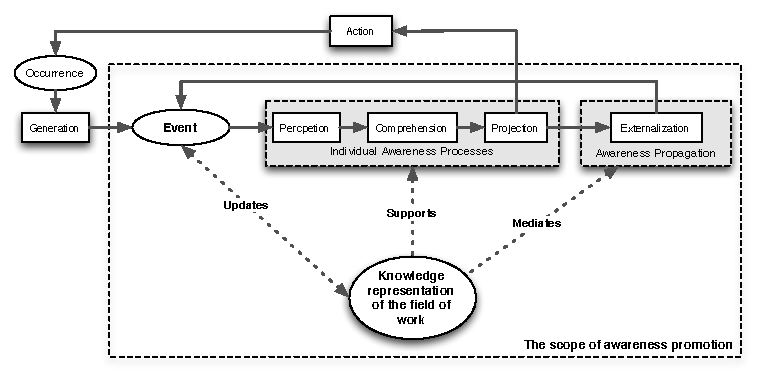
\includegraphics{awareness_promotion_framework.pdf} 
   \caption{Awareness promotion framework}
   \label{fig:awareness_promotion_framework}
\end{figure}

On one hand is how the computer constructs and develops the knowledge representation of the collaborative activities within the event-driven processes. In order to model the development of collaborative activities, the computational representation should support dynamic adaptation so that it always reflects the current state of the changing environment. As human actors use a subset of the awareness information to develop their individual awareness, the system processes the awareness information that is available in the whole collaborative activity. The awareness information can be generated by sensing the occurrences in real world, or it can be the results of human actors' externalization of their individual awareness. All of the awareness information will be processed by the computer system to update its knowledge representation of the collaborative activity.

On the other hand, the knowledge representation is used by the computer system to promote the awareness processes. In general, the role of the computer system is to strike a balance between the system's reasoning capabilities and providing visual and interactive support. With the computational knowledge about the collaborative activities, the system can offload some of the reasoning effort from the human actors. Meanwhile, the systematic knowledge can also be visualized to help the human actors to develop their individual awareness or externalize it for awareness transactions. 

Following of this section discusses the major design choices of these two components, but leave their details to next two chapters respectively.

\subsection{Computational knowledge representation} % (fold)
\label{sub:computational_knowledge_representation}
The nature of awareness phenomena in distributed, complex collaboration as we conceptualized in Section \ref{cha:the_conceptual_framework}, and the goal of promoting awareness impose several requirements for the knowledge representation of the collaborative activity:

\begin{enumerate}
   \item The representation should encode enough knowledge about collaborative activities, including all the three constructs in our conceptual model, i.e. the basic elements and relations in collaborative activities, the local scopes of work for actors, and the various dependency relationships among actions. 
   \item The knowledge representation should be dynamically updated. Since the awareness needs of users change quickly with the development of collaborative activities, it is essential that the knowledge representation should be kept updating so that it always reflects the current state of the changing activities.
   \item The knowledge representation needs to be formalized and can be computationally modeled so as to support reasoning.
\end{enumerate}

Existing awareness systems have provided several approaches to representing the collaborative work. The AREA system \cite{fuchs1999a} models the collaborative work as semantic networks including relations among objects, where objects can be human actors artifacts, or aggregations such as groups of people. The representation is primarily used for the users to specify which objects and associated events they are interested in and when they want to be informed. The Atmosphere model \cite{Rittenbruch2002} describes the collaborative work as a hierarchically structured workspace that consists of a set of \emph{spheres} and \emph{sub-spheres}. Users classify their actions on artifacts by mapping them into different spheres. The MoMA model \cite{simone2002a} applies a reaction-diffusion metaphor to model the collaborative work as a set of entities embedded in an interaction space, which behave by using diffusion and reaction capabilities. This metaphor is based on the idea that whenever two or more entities have contact, their states are modified in some way. Their states are then propagated to others through fields in the space.  

Although these representations have shown their capabilities to support specific aspects of awareness in their respective application domains, none of them can meet all the three requirements for knowledge representation to enable awareness promotion. The AREA model provides a good representation of the actions and the dependencies using the semantic networks, but the local scopes of actors are not captured. The model is static (as it is pre-determined by the designers), and informal (as it is primarily used as a descriptive framework). The Atmosphere model organizes the field of work around the artifacts without explicit representation of actions. It supports the specification of each user's local scope using private `spheres', but no dependency relationships between actions are supported. It supports the modification to the representation by human users, but the system cannot automatically adapt the representation to the changing environment. The MoMA model can support all the three constructs of the field of work as the definition of entities and spaces are generic, and provide some reasoning capabilities. However, it does not support the dynamical adaptation of the model.

In this study we draw knowledge representation and reasoning techniques from existing studies in artificial intelligence to develop a computational model of the collaborative activities that can satisfy all the three requirements. An important feature of our model is the capability to model intentions, beliefs, knowledge, and other attributes of actors' mental states \cite{grosz1996collaborative}. As human actors' awareness processes are directed by their mental models, we believe that understanding and representing human actors' mental states allow the computer to infer each actor's local scope, and derive awareness needs from it. 
% subsection computational_knowledge_representation (end)

\subsection{Event driven awareness processes} % (fold)
\label{sub:event_driven_awareness_processes}
In our approach, we adopt the general event-driven interaction paradigm \cite{Etzion2010} to model the awareness processes. In the event-driven mode of interaction, actors (both human and computer) communicate by generating and receiving events. Each actor receives events from environment and other actors, reacts to them, and generates new events to other actors. We believe that the event-driven paradigm is suitable for modeling awareness processes in our study for two major reasons:

\begin{enumerate}
   \item The event-driven paradigm opens up the opportunities for active promotion by the computational system. Instead of asking the human actors to monitor the environment and pull awareness information from it, events are pushed to them. The information push allows the system to take control and present the awareness information to the actors before they subscribe to them.
   \item As awareness information is explicitly represented as first-class objects in event-driven approaches, this allows for representing any aspects of the collaborative activities, not only the external aspects, but also the internal aspects reflecting intentions and beliefs of the actors.
\end{enumerate}

\subsubsection{The concept of event} % (fold)
\label{ssub:the_concept_of_events}
Before going further we should clarify what we mean by an event. The concept of `event' has been used in the literature from different perspectives:

\begin{enumerate}
   \item The first meaning refers to an actual occurrence (the something that has happened) in the real world. Set out by Quine \cite{quine1985events}, events in this meaning are first-class entities that can be localized in space and time, broken into sub-parts, and arranged in a taxonomic hierarchy. Research using this concept of events primarily focuses on studying the internal structures of the events. For example, in \cite{Yuan2001}, complex geographical phenomena, such as wildfire or precipitation, have been modeled in a hierarchy of events, processes, and states. In \cite{Andrienko2011}, the event-based approach has been adopted to model all the types of occurrences in movement analysis. The focus here is to derive the different event types that may occur and identify the relationships between them.
   \item The second meaning takes us into the realm of computerized event processing, where the word `event' is used to mean a programming entity that represents this occurrence \cite{Spiteri2000}. Each event in this notion is a message that describes a real world occurrence by its source, location, time, and other measurable properties. A single event occurrence can be represented by many event entities, and a given event entity might capture only some of the facets of a particular event occurrence \cite{Etzion2010}.
   \item In event-based awareness systems, the concept of event has a more specific meaning as representing a specific type of awareness information that might be relevant to the user's work. It is usually an application-specific concept, depending on the set of awareness information that is supported by an awareness system. For instance, the AREA system \cite{fuchs1999a} describes events as actions performed on an artifact and the event classes are derived from the artifact class hierarchy and possible operations on them. The ENI system \cite{Gross2004} describes events from the sensors associated with actors, shared artifacts, or any other objects that generate events related to them. 
\end{enumerate}

In this study, we use three different words to avoid the confusion when defining events:
\begin{enumerate}
   \item We use the word \emph{`occurrence'} to denote the real world happenings. It can be in the environment, e.g. the occurrence of a traffic accident at a location; or associated with an object, e.g. a vehicle arrives at the accident spot; or associated with human actions, e.g. the successful performance of first aid on a victim. 
   \item The word \emph{`awareness'} is used to refer to the human consciousness about the occurrences, events, and their relevance to ongoing or future human activities. It emphasizes that awareness is inherently a cognitive, interpretive, and predicative concept that reflects a state of mind.
   \item We use the word \emph{`event'} to denote a computerized entity that describes a piece of awareness information that is relevant to an actor's work. On one hand, it can be the description of a real world \emph{occurrence} by its measurable properties, e.g. the information about a traffic accident with time, location, number of victims etc. On the other hand, it can also be the externalization of an actor's \emph{awareness} knowledge, e.g. an actor's belief that the accident will block the traffic and cause a delay on delivery of medical team.
\end{enumerate}
% subsubsection the_concept_of_event (end)

\subsubsection{Awareness processes} % (fold)
\label{ssub:awareness_processes}
Along with the distinction between the concepts of \emph{`occurrence'}, \emph{`awareness'}, and \emph{`event'} is the notion of dynamic transformations between them (Figure \ref{fig:occurrence_event_awareness}). The transformations are tied to different processes in awareness development. 

\begin{figure}[htbp] %  figure placement: here, top, bottom, or page
   \centering
   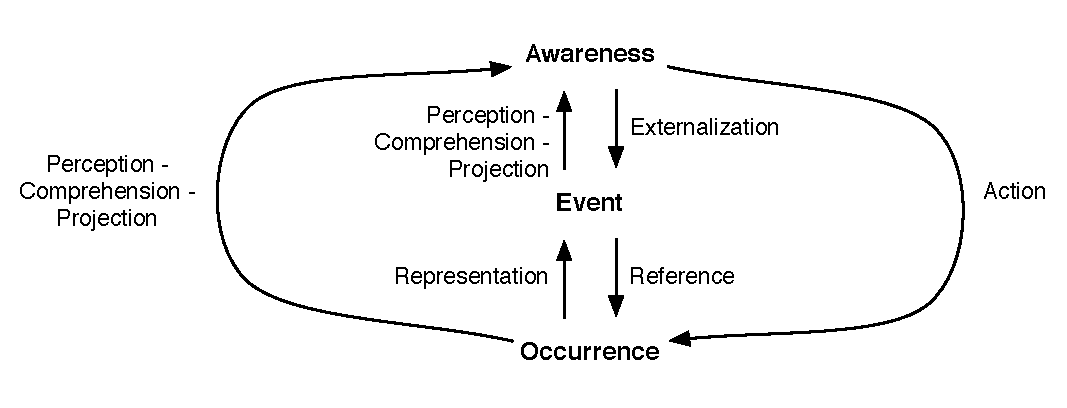
\includegraphics[width=4.5in]{occurrence_event_awareness.pdf} 
   \caption{Transformations between occurrence, event, and awareness}
   \label{fig:occurrence_event_awareness}
\end{figure}

The direct transformation between \emph{occurrence} and \emph{awareness} corresponds to the individual awareness development cycle that has been described in Section \ref{sec:development_of_awareness}. A real world \emph{occurrence} is transformed into \emph{awareness} through an actor's individual awareness processes, i.e. \emph{perception}, \emph{comprehension}, and \emph{projection}. Then, the achieved \emph{awareness} guides the actor's \emph{action} that may generate further \emph{occurrences} in the real world. 

The thing becomes more interesting when the computer support is involved and the transformations are driven by \emph{events}. On one hand is a real world \emph{occurrence} can be captured and represented as an \emph{event} by the computer system, and presented to a human actor. Instead of perceiving the \emph{occurrence} directly, the actor perceives the corresponding \emph{event} in the computer interface, and develops the \emph{awareness} upon it through the actor's individual awareness processes, i.e. \emph{perception}, \emph{comprehension}, and \emph{projection}. On the other hand is some aspect of the actor's \emph{awareness} can be externalized as a new \emph{event}, which refers to some current \emph{occurrence} or predicts future \emph{occurrence} in the real world.

The event-driven transformations can also be used to describe the different types of awareness transactions across multiple actors. The process of \emph{mutual monitoring} can then be described in the following steps: (1) an actor's \emph{awareness} guides his/her \emph{action} that generates a new \emph{occurrence} in the real world; (2) this new \emph{occurrence} is then captured and represented as an \emph{event} by the computer, and presented to another actor; (3) the other actor develops the \emph{awareness} upon receiving the new event. Similarly, the process of \emph{externalization} can also be described as follow: (1) an actor's \emph{awareness} is externalized as a new \emph{event}, which refers to some current \emph{occurrence}; (2) this new \emph{event} is then presented to another actor by the computer; (3)the other actor develops the \emph{awareness} upon receiving the new event. 

Figure \ref{fig:example_awareness_traj} shows an example of how these event-driven awareness processes can be combined together to describe a developmental trajectory of awareness that involves three actors in a group. The awareness is propagated from $Actor1$ to $Actor2$ through the process of \emph{externalization}, and is then propagated from $Actor2$ to $Actor3$ through the process of \emph{mutual monitoring}.

\begin{figure}[htbp] %  figure placement: here, top, bottom, or page
   \centering
   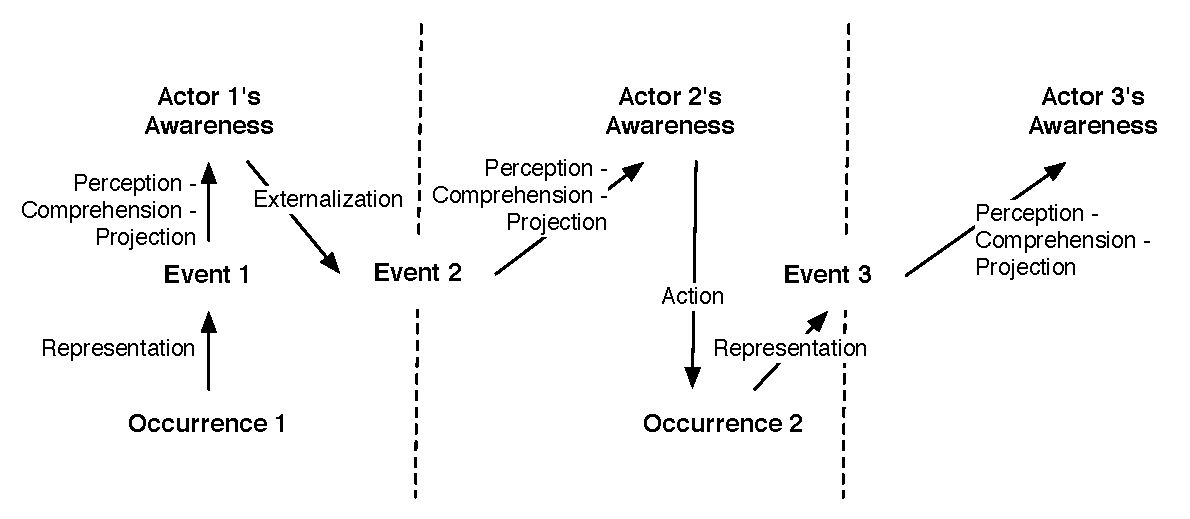
\includegraphics[width=4.5in]{example_awareness_traj.pdf} 
   \caption{An example of event-driven developmental trajectory}
   \label{fig:example_awareness_traj}
\end{figure}
% subsubsection awareness_processes (end)
% subsection event_driven_awareness_processes (end)
% section the_awareness_promotion_framework (end)

\section{Discussion} % (fold)
\label{sec:discussion}
Motivated by the limitations of existing awareness support systems, in this chapter we argue that the computer system needs to play a more active role to promote awareness among collaborators, and provide an overview of the awareness promotion approach. We believe the characteristics of awareness promotion approach provide the potential to address limitations of existing awareness systems to handle the scaled-up complexity and dynamics, and to provide integrated awareness support. First, the awareness promotion approach utilizes the computational knowledge representation to model the collaborative activities and offloads some of the representation and reasoning efforts from the human to the computer. Hence, it can  handle more complex collaborative configurations than existing awareness models. Meanwhile, the knowledge representation is dynamically updated to reflect the current state of the collaborative work, which allows it to handle increased level of dynamics. Last, as the computer's knowledge representation is at the team level and is equipped with the computational reasoning capabilities, it allows the computer to provide support on both the higher level of individual awareness processes and awareness transactions.

The next two chapters provide details of this awareness promotion framework. Chapter \ref{cha:knowledge_reprsentation_and_updating} describes the knowledge components, i.e. the computational representation of the collaborative activities and the specification of events, and the mechanisms for updating the knowledge representation with events. Chapter \ref{cha:promoting_event_driven_awareness} describes the different promotion strategies making use of the knowledge representation.
% section discussion (end)
% chapter awareness_promotion (end)




 

